\documentclass[ShortAfour]{sage}

\usepackage{amsthm,amssymb,url,amsmath}
\usepackage{tipa}
\usepackage{xcolor}%color
\usepackage{bm}
\usepackage{booktabs}
\usepackage{textcomp}
\usepackage[colorlinks,linkcolor=black,anchorcolor=black,citecolor=black]{hyperref}
\usepackage{amsfonts}
\usepackage{color,soul}
\usepackage{subfigure}
\usepackage[square]{natbib}
\theoremstyle{plain}
\newtheorem{myas}{Assumption}
\newtheorem{mydef}{Definition}
\newtheorem{mylem}{Lemma} 
\newtheorem{mythm}{Theorem}
\newtheorem{mypro}{Property}

%\theoremstyle{remark}
\theoremstyle{remark}
\newtheorem{myrem}{Remark}
\newtheorem{mycase}{Case}
\newtheorem{mycase1}{Case}

%\newcommand{\vector}[1]{${#1}_1,{#1}_2,\cdots,{#1}_n$}
\newcommand{\mycolor}[2]{{\color{#1}#2}}


%%%%%%%%%%Harvard or vancouvar style use the following
%%style file natbib.sty package
%\usepackage[numbers,sort&compress]{natbib}
%\bibpunct[, ]{(}{)}{,}{a}{}{,}
 % Use \bibpunct with 6 mandatory arguments:
 %    1. opening bracket for citation
 %    2. closing bracket
 %    3. citation separator (for multiple citations in one \cite)
 %    4. the letter n for numerical styles, s for superscripts
 %        else anything for author-year
 %    5. punctuation between authors and date
 %    6. punctuation between years (or numbers) when common authors missing
 % One optional argument is the character coming before post-notes. It
 %   appears in square braces before all other arguments. May be left off.
 % Example (and default) \bibpunct[, ]{(}{)}{;}{a}{,}{,}
%%%%%%%%%%%%%%%%%%%%%%%%%%%%%%%%%%%%%%%%%%%%%%%%%%%%%%%%%%%%%%%%%%%%%%%%%%%
%%There are two example reference database sample is given
%%as sage_harvard.bib and sage_vancouvar.bib
%%Use these two files, we update the reference entries into these database file






%%%Ref. information%%%%%%%%%%%%%%%%%%%%%%%%%%%%%%%%
\journal{Proc IMechE Part G: Journal of Aerospace Engineering}
\volume{000}
\issue{00}
\copyrightline{$\copyright$ Copyright}
\firstpage{1}
\lastpage{21}
\doi{doi number}
\articletype{Article type}
\pubyear{2018}
%%%%%%%%%%%%%%Article information%%%%%%%%%%%%%%%%%%%%%%%%


\markboth{Running head left side}{Running head right side}


\begin{document} 



%\title{Universal integral sliding mode control for deployment of tethered spacecraft system}
\title{ Fractional order sliding mode control for deployment of tethered spacecraft system}

\author{Zhiqiang Ma\thanks{Corresponding author;
e-mail: zhiqiangma@nwpu.edu.cn}}

\address{National Key Laboratory of Aerospace Flight Dynamics and Research Center for Intelligent Robotics, School of Astronautics, Northwestern Polytechnical University, Xi'an 710072, China}

\author{Zheng H. Zhu} 

\address{Department of Mechanical Engineering, York University, Toronto, Ontario M3J 1P3, Canada}

\author{Guanghui Sun}

\address{Research Institute of Intelligent Control and Systems, Harbin Institute of Technology, Harbin 150001, China}



\maketitle

\begin{abstract}
  This paper proposes a fractional order integral sliding mode control with the order $0<\nu<1$ to stabilize the deployment of tethered spacecraft system with only tension regulation. 
  The work in this paper is partially based on integer-order nonlinear sliding mode controller and improves its performance with fractional order calculus. 
  The proposed scheme makes use of integral sliding surface to obtain smaller convergence regions of state errors, and the fractional derivate is synthesized to enhance the flexibility of controller design by fining parameters for better dynamic and steady-state performance. 
  Fractional order observers help to eliminate external disturbances while the adaptive law is presented to remove the adverse effect in stability analyses, and fractional order uniform ultimate boundedness is proved to guaranteed the existence of proposed sliding surface. According to theoretical analyses, the fractional order will indeed affect the dynamic and steady-state performance of control system, and the proposed method will be verified in numerical simulations compared with the nonlinear sliding mode counterpart.
\end{abstract}

\keywords{Tethered spacecraft systems; sliding mode control; fractional order systems; input constraint}


\section{Introduction}

Tethered spacecraft systems (TSS) have been widely studied to verify its feasibility in simulations and practicability in space experiments. Deployment process of TSS is aimed at driving subspacecraft onto specified orbit, and it is hence an essential stage to start a space mission, such as maneuvering of TSS, formation flight, tether-based capture and re-entry capsule~\cite{huang_wang_meng_liu_2015,Williams2009745,Steindl2016,mantellato2017simulation,ASLANOV2017180}. 
It is noted that deployment dynamics and control is one of the most key issues in these mentioned tasks, and many advanced control strategies have been proposed to achieve a stable and fast deployment~\cite{wen2016constrained,Ma2017Pure}. 

In general, there exist two typical difficult problems to deal with in controller design for deployment, and they are underactuated dynamics and constrained input when only using tension.
To address the complicated inplane dynamics, Sun~{\it et al.} reported a fractional order control law based on linearized model, and illustrated the root distribution to indicate that the stability condition for an integer-order control law is a subset of its fractional-order counterpart~\cite{sun2014fractional,sun2014fractional-order}. 
The analytical deployment control law on account of $J_2$ perturbation, air drag force, and solar pressure was proposed by Yu~{\it et al.}~\cite{yu2017analytical}, which presented the necessary and sufficient conditions of parameter domains for tensile state of space tether.
Mission function based feedback control is specified for the control problem of the TSS, and Kojima~{\it et al.} developed the mission function by considering the difference in original model~\cite{kojima2015mission}. 
Optimal control is a comprehensive method by viewing the deployment process as a nonlinear optimization problem, where the constrained tension was designed as the terminal condition and the underactuated dynamics can be evaluated by a cost function indirectly, and it has hence been thought of as one of the most high effective solutions~\cite{wen2015space}. 


Alongside previous advanced works mentioned above, sliding mode control has been proven to own some advantages to facilitate deployment process due to its robustness to disturbance, low sensitivity to parametric uncertainties and flexible design with other algorithms~\cite{MA2017355}. 
Ref.~\cite{MA201667} linearized the model to utilize linear sliding mode methodology to generate stable reduced order system, and the input constraint was coped with an adaptive law based on Lyapunov second method. 
To accelerate the deployment process, Zhao~{\it et al.} utilized super-twisting technique to reform the sliding surface for desired performance~\cite{zhao2018dynamic}. 
Kang~{\it~et~al.} developed a fractional order sliding surface to govern the reduced order system by tuning the fractional order to improve the deployment performance, and it is noted that this approach was also based on the linearized reduced order system which is much simpler than the nonlinear counterpart~\cite{KANG2017263}. 
To present the high accurate deployment dynamics, Ma~{\it et al.} designed a nonlinear sliding surface to generate a rigorous nonlinear reduced order system, and well analysed the stability of the motion on the surface. They used an adaptive method to produce the constraint tension control strategy, and solved the underactuated dynamics by reconstructing reduced order system with virtual disturbance consisting of actuated dynamics~\cite{Ma2017Pure}. The results in Ref.~\cite{Ma2017Pure} showed that the adverse effect caused by constrained input may propagate to the reduced order system and degenerate the steady-state performance.
 
Integral operator can well suppress the steady-state error and has enabled a wide scope of application areas including control in robotics,  electric drives, etc.~\cite{Utkin1996}. 
In addition, fractional order calculus can be introduced to enhance the flexibility of controller design to make their constructs more accurate~\cite{sun2018practical,sun2018discrete,sun2017practical}. Due to the nature of fractional order calculus, the fractional order sliding surface specified for integer-order systems will lead to some residual errors in stability analysis, and the boundedness of  fractional order systems with uncertainties has not been well analyzed. 

Motivated by the advantages of fractional order calculus and based on previous works, to deal with the underactuated dynamics and constrained tension, a fractional order sliding mode control for the deployment of tethered spacecraft systems is proposed in this paper. For more accurate dynamics, a novel nonlinear fractional integral sliding surface is presented to establish a stable reduced order fractional order system due to fractional order uniform ultimate boundedness that is discussed in this paper for the first time, and the corresponding disturbance observers are designed by using fractional order calculus to eliminate the external disturbances while the fractional order adaptive law works to remove the adverse effect in stability analysis. The novelty of this work is to allow an adjustable fractional order as a parameter to tune in the control system for seeking a better dynamic and steady-state performance. Moreover, the fractional order sliding mode controller is rigorous nonlinear, consisting of fractional derivate and integral. The remainder of this paper is organized as follows: Section~\ref{sec:mm} will introduce the deployment dynamics, the corresponding integer-order nonlinear controller design and the new fractional order sliding mode controller design, and analyze the fractional order uniform ultimate boundedness of deployment dynamics. Section~\ref{sec:numerical simulation} will examine the numerical results by tuning fractional order to verify the effectiveness of proposed approaches. Section~\ref{sec:Conclusion} summaries all the works.


\section{Dynamics and control}\label{sec:mm}
In the light of Lagrangian mechanics, the deployment dynamics of TSS can be described by \cite{Williams2009745}
\begin{align} 
\begin{split}
&\theta''+2\left(\theta'+\Omega\right)l'/l+3\Omega^2\sin{\theta} \cos{\theta}=Q_\theta/(\bar{m}l^2)\\
&l''-l\left[\left(\theta'+\Omega\right)^2+\Omega^2\left(3\cos{^2\theta}-1\right)\right]= -\tau/\bar{m}+d\label{eq:motion1}
\end{split}
\end{align}
where $\tau$ denotes the tension acting along the space tether, and the generalized force $Q_\theta$ is related to phase of $\theta$ and is regarded as zero as the tension is the only force to regulate the inplane dynamics. To maintain the space tether taut, the condition $0<\tau_{min}\le \tau\le \tau_{max} < \infty$ should be ensured during the entire liberation, that is, $\tau_{max}$ averts the breakage of space tether and $\tau_{min}>0$ precludes a slack tether. The derivative with respect to time is represented by $()'$, and $d$ represents the disturbance. $\bar m$ is the relative system mass related to the mother spacecraft and the subspacecraft, and $\Omega$ means the orbital angular speed. $l$ and $\theta$ are referred to as the space tether length and the inplane angle, respectively, and these two states together depict the inplane dynamics~\cite{williams2008deployment}.

Introducing the dimensionless conversion Eq.(\ref{eq:varcon}) into Eq.(\ref{eq:motion1}) obtains the normalized formulation of deployment dynamics (\ref{eq:original motion equation}).
\begin{align}
\begin{split}
&\lambda=l/L\\
&d()/dt=\Omega d()/dv\\
&\hat{\tau}=\tau/(\bar{m}\Omega^2L)\\
&d_2 = d/(\bar{m}\Omega^2L)\label{eq:varcon}
\end{split}
\end{align}
where $L$ is the desired length of space tether, and $v = \Omega t$ means the dimensionless time.
\begin{align}\begin{split}
  &\ddot\theta+2\left(\dot\lambda/\lambda\right)\left(1+\dot\theta\right)+3\cos\theta\sin\theta=0\\
  &\ddot\lambda-\lambda\left[\left(1+\dot\theta\right)^2-1+3\cos^2\theta\right]=-\hat T+d_2\label{eq:original motion equation}.
\end{split}\end{align}
It is noted that the dimensionless space tether length is positive. It is worth pointing out that the system (\ref{eq:original motion equation}) is singular before the beginning of the deployment since $\lambda = 0$, and to make the deployment model physically meaningful, the dimensionless space tether length $\lambda$ is artificially initialized with a small positive scalar. In reality, there indeed exists a certain initial distance between the two spacecrafts to avert colliding.

\subsection{Integral sliding mode controller design}
To complete the deployment of subspacecraft, it is required that the space tether to be unreeled as desired length along the local vertical direction, and the desired condition can hence be determined: $\theta_d=\dot\theta_d=0$, $\lambda_d=1$ and $\dot\lambda_d=0$. For the sake of controller design, it is essential to turn the system (\ref{eq:original motion equation}) into an error formulation by
\begin{align}\begin{split}
  e_1 = \theta - \theta_d,\quad e_2 = \dot\theta-\dot\theta_d,\quad
  e_3 = \lambda - \lambda_d,\quad e_4 = \dot\lambda-\dot\lambda_d,\label{eq:error}
\end{split}\end{align}
and substituting Eq.(\ref{eq:error}) into system (\ref{eq:original motion equation}) yields
\begin{align}\begin{split}
  \dot e_1 &= e_2\\
  \dot e_2 &= f_1(e_1,e_2,e_3,e_4)+d_1\\
  \dot e_3 &= e_4\\
  \dot e_4 &= f_2(e_1,e_3,e_3,e_4)+u+d_2\label{eq:nominal model},
\end{split}\end{align}
where
\begin{align}\begin{split}
  f_1(e_1,e_2,e_3,e_4) &= -\frac{2e_4(1+e_2)}{e_3+1}-3\cos e_1\sin e_1-\varepsilon e_3\\
  f_2(e_1,e_3,e_3,e_4) &= (e_3+1)\left[(1+e_2)^2-1+3\cos^2 e_1\right],
\end{split}\end{align}
and $d_1=\varepsilon e_3$ is constructed as a virtual disturbance. Owing to the presence of the virtual disturbance, it is clear to prove that $f_1(0,0,e_3,e_4)$ is specified to be asymptotically stable by combing with the third row of Eq.(\ref{eq:nominal model}). According to the physical feature of the tension, the input in system (\ref{eq:nominal model}) is strictly constrained and is expressed by
\begin{align}
  u_c = u - \Delta u\label{eq:delta u}
\end{align}
where $u_c$ is the control command generated by controller, while $u$ is the actual input given out by the actuator.
For the subsequent entire controller design, we have the following assumption and lemmas for system (\ref{eq:nominal model}).
\begin{myas}
To achieve a smooth deployment, the angular rate with $\dot\theta+1>0$ should be satisfied. In this regard,  $\partial f_1/\partial e_4$ is invertible, while this assumption precludes the singularity of the subsequent controller design. The disturbances are assumed to be bounded with $\left\vert\dot d_1\right\vert\le \rho_1$, $\left\vert \dot d_2\right\vert\le \rho_2$, $\left\vert d_3\right\vert\le \rho_3$, $\left\vert d_4\right\vert\le \rho_4$ and $\rho_i>0,i = 1,2,3,4$.
\end{myas}
\begin{mylem}\cite{Do2010}
  Consider a second order system:
  \begin{align}\begin{split}
    \dot x_1 &= x_2\\
    \dot x_2 &= f(x_1,x_2,u)+d
  \end{split}\end{align}
where $f(x_1,x_2,u)$ is known function, and $d$ is bounded with $\left\vert\dot d\right\vert<C_d$. The construction of disturbance observer can achieve that the estimator error $\tilde d = (\hat d-d)$ exponentially converge to the a ball centered at the origin, and the ball can be made arbitrarily small by suitable selection of the parameters.
\begin{align}\begin{split}
  \hat d &= q+kx_2\\
  \dot q &= -kq-k(f(x_1,x_2,u)+kx_2)
\end{split}\end{align}
where $k$ is a positive scalar.
\end{mylem}
\begin{myrem}
  Based on the above lemma and system (\ref{eq:nominal model}), we can design the following observers to compensate the negative effect of disturbances.
  \begin{align}\begin{split}
    \dot q_1 &= -k_1q_1-k_1(f_1+k_1e_2)\\
    \hat d_1 &= q_1+k_1e_2\label{eq:do1},\\
  \end{split}\\
  \begin{split}
      \dot q_2 &= -k_2q_2-k_2(f_2+u+k_2e_4)\\
      \hat d_2 &= q_2+k_2e_4\label{eq:do2},\\
  \end{split}\end{align}
  where $k_1>0$, $k_2>0$, $q_1$ and $q_2$ are auxiliary variables of the disturbance estimators $\hat d_1$ and $\hat d_2$, respectively.
\end{myrem}
\begin{mylem}\cite{Chen2011}\label{lem: adaptive input}
  To cope with the input constraint, the auxiliary dynamic system (\ref{eq:adaption}) is employed to guarantee the valid stability analysis.
  \begin{align} \dot\eta=\left\{
  \begin{aligned}
  &-k_3\eta-\frac{(\partial f_1/\partial e_4)s_i\Delta u+\frac{1}{2}(\Delta u)^2}{\eta^2}\eta+\Delta u,\quad&\vert\eta\vert\ge\sigma \\
  &0,\quad&\vert\eta\vert<\sigma \end{aligned}
  \right.,\label{eq:adaption}
  \end{align}
where $k_3>0$ and $\sigma$ is a small positive scalar.
\end{mylem}


Regarding Eq.(\ref{eq:delta u}) and the external disturbance, a trivial integral sliding mode surface can be designed as
\begin{align}\begin{split}
  s&=c_1e_1+c_2e_2+f_1\\
  s_i&=s+\chi\\
  \dot\chi&=s\label{eq:integral sliding surface}
\end{split}\end{align}
and in accordance with Eq.(\ref{eq:do1}), Eq.(\ref{eq:do2}), Eq.(\ref{eq:adaption}) and Eq.(\ref{eq:integral sliding surface}), the controller input can be constructed as
\begin{align}\begin{split}
  u_c =& -\left(\frac{\partial f_1}{\partial e_4}\right)^{-1}\left(s+c_1e_2+c_2f_1+\frac{\partial f_1}{\partial e_1}e_2+\frac{\partial f_1}{\partial e_2}f_1+\frac{\partial f_1}{\partial e_3}e_4+\frac{\partial f_1}{\partial e_4}f_2\right)\\
  &-\left(\frac{\partial f_1}{\partial e_4}\right)^{-1}k_4s_i-\hat d_2-\left(\frac{\partial f_1}{\partial e_4}\right)^{-1}\left(c_2+\frac{\partial f_1}{\partial e_2}\right)\hat d_1-k_5\left(\frac{\partial f_1}{\partial e_4}\right)^{-1}\eta\label{eq:uc}
\end{split}\end{align}
to ensure that the system state errors are all uniformly ultimately bounded.

Select the Lyapunov function candidate
\begin{align}
  V_i = \frac{1}{2}s_i^2+\frac{1}{2}\tilde d_1^2+\frac{1}{2}\tilde d_2^2+\frac{1}{2}\eta^2,\label{eq:v}
\end{align}
and its derivative is
\begin{align}
  \dot V_i = s_i(\dot s+s)+\tilde d_1\dot{\tilde d}_1 +\tilde d_2\dot{\tilde d}_2+\eta\dot\eta\label{eq:dv}.
\end{align}
In the light of Eq.(\ref{eq:integral sliding surface}), Eq.(\ref{eq:uc}) and Young's inequality, one can obtain
  \begin{align}\begin{split}
    s_i\dot s_i&=s_i\left[-k_4s_i-\frac{\partial f_1}{\partial e_4}\hat d_2+\frac{\partial f_1}{\partial e_4}d_2-\left(c_2+\frac{\partial f_1}{\partial e_2}\right)\hat d_1+\left(c_2+\frac{\partial f_1}{\partial e_2}\right)d_1+\frac{\partial f_1}{\partial e_4}\Delta u-k_5\eta\right]\\
    &=-k_4s_i^2+\frac{\partial f_1}{\partial e_4}s_i\tilde d_2 +\left(c_2+\frac{\partial f_1}{\partial e_2}\right)s_i\tilde d_1+\frac{\partial f_1}{\partial e_4}s_i\Delta u-k_5\eta s_i\\
    &\le -k_4s_i^2+\frac{1}{2}\left\vert\frac{\partial f_1}{\partial e_4}\right\vert s_i^2+\frac{1}{2}\left\vert\frac{\partial f_1}{\partial e_4}\right\vert \tilde d_2^2+\frac{1}{2}\left\vert c_2+\frac{\partial f_1}{\partial e_2}\right\vert s_i^2+\frac{1}{2}\left\vert c_2+\frac{\partial f_1}{\partial e_2}\right\vert \tilde d_1^2+\frac{1}{2}s_i^2+\frac{1}{2}k_5^2\eta^2+\frac{\partial f_1}{\partial e_4}s_i\Delta u\\
    &\le -\left(k_4-\frac{1}{2}\left\vert\frac{\partial f_1}{\partial e_4}\right\vert-\frac{1}{2}\left\vert c_2+\frac{\partial f_1}{\partial e_2}\right\vert-\frac{1}{2}\right)s_i^2+\frac{1}{2}\left\vert\frac{\partial f_1}{\partial e_4}\right\vert\tilde d_2^2+\frac{1}{2}\left\vert c_2+\frac{\partial f_1}{\partial e_2}\right\vert\tilde d_1^2+\frac{1}{2}k_5^2\eta^2+\frac{\partial f_1}{\partial e_4}s_i\Delta u.\label{eq:sds}
  \end{split}\end{align}
Using Eq.(\ref{eq:do1}), Eq.(\ref{eq:do2}) and Young's inequality results in
\begin{align}\begin{split}
  \tilde d_1\dot {\tilde d}_1+\tilde d_2\dot {\tilde d}_2&=-k_1\tilde{d}_1^2- \dot d_1\tilde{d}_1-k_2\tilde{d}_2^2- \dot d_2\tilde{d}_1\\
  &\le-\left(k_1-\frac{1}{2}\right)\tilde{d}_1^2+ \frac{1}{2}\dot d_1^2-\left(k_2-\frac{1}{2}\right)\tilde{d}_2^2+ \frac{1}{2}\dot d_2^2\\
  &\le-\left(k_1-\frac{1}{2}\right)\tilde{d}_1^2-\left(k_2-\frac{1}{2}\right)\tilde{d}_2^2+ \frac{1}{2}\rho_1^2+ \frac{1}{2} \rho_2^2.\label{eq:d1d1+d2d2}
\end{split}\end{align}
One can proceed the stability analysis according to the different range which $\eta$ is located in.
\begin{mycase}
  When $\vert\eta\vert\ge\sigma$, introducing Eq.(\ref{eq:adaption}), Eq.(\ref{eq:sds}) and Eq.(\ref{eq:d1d1+d2d2}) into Eq.(\ref{eq:dv})  obtains
  \begin{align}\begin{split}
    \dot V_i \le &-\left(k_4-\frac{1}{2}\left\vert\frac{\partial f_1}{\partial e_4}\right\vert-\frac{1}{2}\left\vert c_2+\frac{\partial f_1}{\partial e_2}\right\vert-\frac{1}{2}\right)s_i^2-\left(k_1-\frac{1}{2}-\frac{1}{2}\left\vert c_2+\frac{\partial f_1}{\partial e_2}\right\vert\right)\tilde{d}_1^2\\
    &-\left(k_2-\frac{1}{2}-\frac{1}{2}\left\vert\frac{\partial f_1}{\partial e_4}\right\vert\right)\tilde{d}_2^2-\left(k_3-\frac{1}{2}k_5^2-\frac{1}{2}\right)\eta^2+\frac{1}{2}\rho_1^2 +\frac{1}{2}\rho_2^2\\
    \le& -2\mu_1V+\Phi_1,\label{eq:dv1}
  \end{split}\end{align}
  where
  \begin{align}\begin{split}
    \mu_1 =& \min\left\{k_4-\frac{1}{2}\left\vert\frac{\partial f_1}{\partial e_4}\right\vert-\frac{1}{2}\left\vert c_2+\frac{\partial f_1}{\partial e_2}\right\vert-\frac{1}{2},k_1-\frac{1}{2}-\frac{1}{2}\left\vert c_2+\frac{\partial f_1}{\partial e_2}\right\vert,\right.\\
    &\left. k_2-\frac{1}{2}-\frac{1}{2}\left\vert\frac{\partial f_1}{\partial e_4}\right\vert,k_3-\frac{1}{2}k_5^2-\frac{1}{2}\right\}>0\\
    \Phi_1=&\frac{1}{2}\rho_1^2 +\frac{1}{2}\rho_2^2.
  \end{split}\end{align}
\end{mycase}
\begin{mycase}
  When $\vert\eta\vert<\sigma$, introducing Eq.(\ref{eq:adaption}), Eq.(\ref{eq:sds}) and Eq.(\ref{eq:d1d1+d2d2}) into Eq.(\ref{eq:dv})  obtains
  \begin{align}\begin{split}
    \dot V_i \le&-\left[k_4-\frac{1}{2}\left\vert\frac{\partial f_1}{\partial e_4}\right\vert-\frac{1}{2}\left\vert c_2+\frac{\partial f_1}{\partial e_2}\right\vert-\frac{1}{2}\left(\frac{\partial f_1}{\partial e_4}\right)^2-\frac{1}{2}\right]s_i^2-\left(k_1-\frac{1}{2}-\frac{1}{2}\left\vert c_2+\frac{\partial f_1}{\partial e_2}\right\vert\right)\tilde{d}_1^2\\
    &-\left(k_2-\frac{1}{2}-\frac{1}{2}\left\vert\frac{\partial f_1}{\partial e_4}\right\vert\right)\tilde{d}_2^2 +\frac{1}{2}k_5^2\sigma^2+\frac{1}{2}(\Delta u)^2+\frac{1}{2}\rho_1^2+\frac{1}{2}\rho_2^2\\
    \le& -2\mu_2V+\Phi_2
  \end{split}\end{align}
  where
  \begin{align}\begin{split}
    \mu_2&=\min\left\{k_4-\frac{1}{2}\left\vert\frac{\partial f_1}{\partial e_4}\right\vert-\frac{1}{2}\left\vert c_2+\frac{\partial f_1}{\partial e_2}\right\vert-\frac{1}{2}\left(\frac{\partial f_1}{\partial e_4}\right)^2-\frac{1}{2},\right.\\
    &\left.k_1-\frac{1}{2}-\frac{1}{2}\left\vert c_2+\frac{\partial f_1}{\partial e_2}\right\vert,k_2-\frac{1}{2}-\frac{1}{2}\left\vert\frac{\partial f_1}{\partial e_4}\right\vert\right\}>0\\
    \Phi_2&=\frac{1}{2}\rho_1^2+\frac{1}{2}\rho_2^2+\frac{1}{2}k_5^2\sigma^2+\frac{1}{2}(\Delta u)^2.\label{eq:dv2}
  \end{split}\end{align}
\end{mycase}
Therefore, one has
\begin{align}
  \dot V_i \le -2\mu V_i+\Phi\label{eq:dv3}
\end{align}
with $\mu =\min\left\{\mu_1,\mu_2\right\}$ and $\Phi =\max\left\{\Phi_1,\Phi_2\right\}$, and one can solve Eq.(\ref{eq:dv3}) to get
\begin{align}
  0\le V_i(t)\le\frac{\Phi}{2\mu}+\left[V_i(0)-\frac{\Phi}{2\mu}\right]e^{-2\mu t}.
\end{align}
With $\mu>0$, the above expression implies
\begin{align}
  0\le\vert s_i(t)\vert\le\sqrt{\frac{\Phi}{\mu}+2\left[V_i(0)-\frac{\Phi}{2\mu}\right]e^{-2\mu t}}\label{eq:abs s}.
\end{align}
One can select the Lyapunov function candidate $V_1=\chi^2$, and along the line of deriving $\vert s_i(t)\vert$, it is easy to obtain
\begin{align}
  0\le\vert \chi\vert\le\sqrt{s_i^2(t)+2\left[V_1(0)-\frac{s_i^2(t)}{2}\right]e^{-t}}\label{eq:chi}
\end{align}
which implies that $\lim\limits_{t\to \infty}\chi$ exists and is bounded. Therefore one has $\lim\limits_{t\to \infty}s=0$ according to Barbalat's lemma. Hence the existence of sliding surface has been proved.
\begin{myrem}
  Utilizing the compensation methods mentioned above to deal with the disturbance and input constraint, compared to the trivial sliding mode control, the integral sliding mode control is capable of reaching the desired sliding surface instead of the boundary layer with a certain thickness.
\end{myrem}
Once the sliding surface is established, the overall system dynamics is handled by the reduced order system
\begin{align}\begin{split}
  \dot e_1 &= e_2\\
  \dot e_2 &= -c_1e_1-c_2e_2+d_1.\label{eq:reduced model}
\end{split}\end{align}
%and to investigate the stability of system, a feasible Lyapunov function candidate can be selected as
%\begin{align}
%V_{2} = \frac{c_1}{2}e_1^2+\frac{1}{2}e_2^2
%\end{align}
%where $V_{2}=0$ if and only if $e_1=0$ and $e_2=0$. Its derivate can be represented by
%\begin{align}\begin{split}
%  \dot V_{2}&=-c_2e_2^2+d_1e_2\\
%  &\le-(c_2-\frac{\rho_3}{\vert e_2\vert})e_2^2.
%\end{split}\end{align}
%In the light of LaSalle's Lagrange stability theorem~\cite{Lasalle1960}, the above expression means that $e_2$ can converge onto the compact set
%\begin{align}
%  \Sigma_1=\left\{e_2\in R\left|\vert e_2\vert\le\frac{\rho_3}{c_2}\right.\right\}\label{eq:sigma1}
%\end{align} which can be arbitrarily small with suitable $c_2$.

For investigating the convergence region of $e_1$, select the Lyapunov function candidate
\begin{align}
  V_2=\frac{1}{2}(c_1-c_2+1)e_1^2+\frac{1}{2}(e_1+e_2)^2
\end{align}
where $c_1>c_2$, and using Young's inequality, the derivate of $V_3$ along the trajectory of Eq.~(\ref{eq:reduced model}) is given by
\begin{align}\begin{split}
  \dot V_2&=-(c_1-c_2+1)e_1^2-\left(c_2-\frac{3}{2}\right)(e_1+e_2)^2+\frac{\rho_3^2}{2}\\
  &\le-2V_2+\frac{\rho_3^2}{2}
\end{split}\end{align}
where $c_2>\frac{5}{2}$. Along the line from Eq.~(\ref{eq:dv3}) to Eq.~(\ref{eq:chi}), $e_1$ can be proved to be uniformly ultimately bounded by
\begin{align}
  0\le\vert e_1(t)\vert\le\sqrt{\frac{\rho_3^2}{2}+2\left[V_3(0)-\frac{\rho_3^2}{4}\right]e^{-2t}}\label{eq:sigma6}
\end{align}
and for convenience of notation, we denote $\vert e_1(t)\vert\le \xi_1$ with $t\to\infty$.
Hence, $e_1$ are both uniformly ultimately bounded and the corresponding convergence precisions are also given out. Moreover, based on Barbalat's lemma, $\lim\limits_{t\to\infty}e_1(t)$ exists and is bounded, $e_2=\dot e_1$ is asymptotically stable. In accordance with the analyses above, with $t\to\infty$, one can proceed to investigate the convergence precision of $e_3$.

Select the Lyapunov function candidate
\begin{align}
  V_3 = \frac{1}{2}e_3^2.
\end{align}

Employing Eq.~(\ref{eq:integral sliding surface}), $e_2+1>0$ and $\lambda = e_3+1>0$, the derivate of $V_3$ can be expressed by
\begin{align}
  \dot V_3 &= -\frac{\varepsilon e_3^2(e_3+1)}{2(e_2+1)}-\frac{e_3(e_3+1)(3\cos e_1\sin e_1-c_1e_1-c_2e_2)}{2(e_2+1)}\\
  &\le -\left(\frac{\varepsilon}{2(e_2+1)}-\frac{\vert 3\cos e_1\sin e_1-c_1e_1-c_2e_2\vert}{\vert2(e_2+1)\vert\vert e_3\vert}\right)e_3^2(e_3+1)
\end{align}
which, according to LaSalle's Lagrange stability theorem~\cite{Lasalle1960}, implies that $e_3$ can converge onto the bound of the compact set $\Sigma_2$ with $t\to\infty$
\begin{align}\begin{split}
  \Sigma_2&=\left\{e_3\in R\left|\vert e_3\vert\le\frac{(2c_1+3)\xi_1}{2\varepsilon}\right.\right\}\label{eq:sigma2}
\end{split}\end{align}
 which can be arbitrarily small with suitable selection of parameters. Therefore, based on Barbalat's lemma, $\lim\limits_{t\to\infty}e_3(t)$ exists and is bounded, and hence $e_4=\dot e_3$ is asymptotically stable.
\subsection{Fractional order sliding mode controller design}\label{sec:fractional controller design} 
At this point, the proof of integral sliding mode control for deployment of tethered spacecraft system has been completed. One can use fractional order calculus to modify the integral controller, that is, the order of sliding surface is designed to be a fraction. To develop the fractional order controller, some fundamental definitions and lemmas are presented previously.
\begin{mydef}[Fractional integral~\cite{Podlubny1999}]
  The fractional integral of function $f(t)$ with order $\nu$ is
  \begin{align}
    _{t_0}D_t^{-\nu} f(t)=\frac{1}{\Gamma(\nu)}\int_{t_0}^t(t-\tau)^{\nu-1}f(\tau)d\tau
  \end{align}
  where $0< \nu< 1$ and $\Gamma(x)=\int_0^\infty e^{-\tau}\tau^{x-1}d\tau$.
  \end{mydef}
\begin{mydef}[Riemann--Liouville fractional derivate~\cite{Podlubny1999}]
For any integrable function $f(t)$, $\nu$-th derivate operator can be defined as
\begin{align}
  ^{RL}_{\ t_0}D_t^\nu f(t)=\frac{1}{\Gamma(1-\nu)}\frac{d}{dt}\int_{t_0}^t(t-\tau)^{-\nu}f(\tau)d\tau
\end{align}
where $0< \nu< 1$.
\end{mydef}
\begin{mydef}[Caputo fractional derivate~\cite{Podlubny1999}]
  For continuously differentiable $f(t):\mathbb R\to \mathbb R$, its fractional order derivative under Caputo definition is
  \begin{align} {}^C_{t_0}D^\nu_tf(t)=
      &\frac{1}{\Gamma(1-\nu)}\int^t_{t_0}\frac{f^{'}(\tau)}{(t-\tau)^{\nu}}d\tau, 
    \end{align}
    where $0<\nu<1$.
  \end{mydef}
\begin{myrem}
  For the convenience of notation, the upper and lower limits of Riemann--Liouville fractional order calculus are omitted during the derivation, and hence $^{RL}_{\ t_0}D_t^\nu f(t)$ equals to $D^\nu f(t)$ if any confusion doesn't occur. It has been proved that $D^\nu\left(D^\beta f(t)\right)=D^{\nu+\beta}f(t)$~\cite{Podlubny1999}.
\end{myrem}
\begin{mylem}[Generalized Mittag--Leffler stability~\cite{Li2009,Li2010}]
  Suppose $V(t,x(t)):[0,\infty)\times D\to R$ with $D\subset R^n$ containing the origin to be a continuously differentiable function and locally Lipschitz with respect to $x$ such that
  \begin{align}
    &\alpha_1\Vert x\Vert^a\le V(t,x(t))\le\alpha_2\Vert x\Vert^{ab}\label{eq:ml c1}\\
    &D^\nu V(t,x(t))\le -\alpha_3\Vert x\Vert^{ab}\label{eq:ml c2}
  \end{align}
  where $t\le 0$ and $x\in D$. $0<\nu<1$, $\alpha_1$, $\alpha_2$, $\alpha_3$, $a$ and $b$ are positive scalars. Hence, one can say $x=0$ is generalized Mittag--Leffler stable.
\end{mylem}
\begin{myrem}
  Generalized Mittag--Leffler stability implies asymptotic stability~\cite{Li2010}. Eq.(\ref{eq:ml c2}) can be written as $D^\beta V(t,x(t))\le -(\nu_3/\nu_2) V$ due to $V(t)\ge 0$.
\end{myrem}
\begin{mydef}~\cite{Podlubny1999}
  Mittag--Leffler function is given by
  \begin{align}
    E_\alpha(z)=\int^\infty_{k=0}\frac{z^k}{\Gamma(k\alpha+1)}
  \end{align}
  where $\alpha>0$. 
  
  Mittag--Leffler function with two parameters is defined as:
  \begin{align}
    E_{\alpha,\beta}(z)=\int^\infty_{k=0}\frac{z^k}{\Gamma(k\alpha+\beta)}
  \end{align}
  where $\alpha>0$ and $\beta>0$. if $\beta=1$, then $E_\alpha(z)=E_{\alpha,\beta}(z)$, and $E_{\alpha=1,\beta=1}(z)=e^z$.
\end{mydef}
\begin{mylem}\cite{Aghababa2014}\label{lem:v}
  If $V(t,x(t))=x^2(t)$ is a continuously differentiable and positive definite function, the fractional order derivative of $V(t,x(t))$ can be given out by
  \begin{align}\begin{split}
    D^\nu V(t,x(t))&=x(t)D^\nu x(t)+\sum^\infty_{i=1}\frac{\Gamma(1+\nu)}{\Gamma(1+i)\Gamma(1-i+\nu)}D^ix(t)D^{\nu-i}x(t)\\
    &\le x(t)D^\nu x(t)+\vartheta\vert x(t)\vert
  \end{split}\end{align}
  where $\vartheta$ is a positive constant.
\end{mylem}
\begin{myas}\label{as:2}
  The disturbance $d_1$ and $d_2$ is assumed to be bounded under the definition of fractional order such that $\left\vert D^\nu d_1\right\vert<\rho_5$ and $\left\vert D^\nu d_2\right\vert<\rho_6$.
\end{myas}

Based on the aforementioned definitions and lemmas, the fractional order calculus can be synthesized into the integer-order sliding mode controller (\ref{eq:uc}) to construct fractional integral sliding mode controller, which can guarantee that all the system state errors are uniformly ultimately bounded.
%\begin{mydef}[Mittag--Leffler functions~\cite{Li2009}]
%  Mittag--Leffler function, regarded as the exponential-like function in fractional order calculus, is frequently used in the solutions of fractional order differential equation and has the following expression
%  \begin{align}
%    E_\nu(z)=\sum^\infty_{k=0}\frac{z^k}{\Gamma(k\nu+1)}
%  \end{align}
%  where $\nu >0$. The two-parameter-type Mittag--Leffler function can be expressed by5
%  \begin{align}
%    E_{\nu,\beta}(z)=\sum^\infty_{k=0}\frac{z^k}{\Gamma(k\nu+\beta)}
%  \end{align}
%  and its Laplace transform is
%  \begin{align}
%    \mathscr{L}\left\{t^{\beta-1}E_{\nu,\beta}(-\lambda t^\nu)\right\}=\frac{s^{\nu-\beta}}{s^{\nu}+\lambda}
%  \end{align}
%  where $\lambda\in R$ and $\mathscr{L}\{\}$ denotes the Laplace transform.
%\end{mydef}

Before the fractional order controller design and stability analyses, the uniform ultimate boundedness of a fractional order system is presented firstly.

\begin{mythm}\label{theorem:fo UUB}
  Considering a nonlinear system $\dot{\bm x}=\bm f(\bm x)+\bm b(t,\bm x)$ with disturbance and uncertainties, $\bm x=0$ is an equilibrium and $\mathbb D\subset \mathbb R^n$ is the vicinity of $\bm x=0$. Selecting a  Lyapunov function candidate $V(t,\bm x(t)):[0,\infty)\times\mathbb D\to \mathbb R$ with $\bm x$ satisfying Lipschitz condition, if one can obtain
  \begin{align}
    \begin{split}\label{eq:ML UUB}
    &\alpha_1\Vert\bm x\Vert^a\le V(t,\bm x(t))\le\alpha_2\Vert\bm x\Vert^{ab}\\
     &^C_{t_0}D_t^\nu V(t,\bm x(t))\le-\alpha_3\Vert\bm x\Vert^{ab}+g(t)
  \end{split}
  \end{align}
  where $t\ge 0$,$\bm x\in \mathbb D$, $\beta\in(0,1)$, $\alpha_1>0$ $\alpha_2>0$, $\alpha_3>0$, $a>0$ and $b>0$. $g(t):[0,\infty)\to \mathcal D$ is the term meaning the bounded disturbance and uncertainties, it results in $V(t,\bm x(t))$ is uniformly ultimately bounded by $\xi$, satisfying
  \begin{align*}
      \xi>\vert g(t)\vert,t\to\infty.
  \end{align*}
  Therefore, $\bm x$ is uniformly ultimately bounded by
  \begin{align*}
      \Vert\bm x\Vert\le \left(\frac{\xi}{\alpha_1}\right)^{\frac{1}{a}},t\to\infty.
  \end{align*}
\end{mythm}
\begin{proof}
In the light of Eq.(\ref{eq:ML UUB}), one has
\begin{align}
  ^C_{t_0} D^\nu_t V(t,\bm x(t))\le -\frac{\alpha_3}{\alpha_2}V(t,\bm x(t))+g(t).
\end{align}
There must exist a function $M(t)>0$ to satisfy
\begin{align}\label{eq:eq Mt}
  ^C_{t_0} D^\nu_t V(t,\bm x(t)) + M(t)= -\frac{\alpha_3}{\alpha_2}V(t,\bm x(t))+g(t)
\end{align}
The Laplace of Eq.(\ref{eq:eq Mt}) can be transformed into
\begin{align}
  s^\nu V(s)-V(0)s^{\nu-1}+M(s)=-\frac{\alpha_3}{\alpha_2}V(s)+g(s)
\end{align}
where $V(0)=V(0,\bm x(0))$, $V(s)=\mathcal L\left\{V(t,\bm x(t))\right\}$. The above equation can be rewritten as
\begin{align}
  V(s)=\frac{V(0)s^{\nu-1}-M(s)+g(s)}{s^{\nu}+\frac{\alpha_3}{\alpha_2}}.
\end{align}

When $\bm x=0$, it is obvious that $V(0)=0$, while $\bm x\neq 0$ leads to $V(0)>0$. Due to the existence of solution of fractional order derivative equation\cite{Podlubny1999}, the solution of $V(t,\bm x(t))$ can be expressed by
\begin{align*}
  V(t)=&V(0)E_\nu\left(-\frac{\alpha_3}{\alpha_2}t^\nu\right)-M(t)\left[t^{\nu-1}E_{\nu,\nu}\left(-\frac{\alpha_3}{\alpha_2}t^\nu\right)\right]\\
  &+g(t)\left[t^{\nu-1}E_{\nu,\nu}\left(-\frac{\alpha_3}{\alpha_2}t^\nu\right)\right]
\end{align*}

Because $t^{\nu-1}$ and $E_{\nu,\nu}\left(-\frac{\alpha_3}{\alpha_2}t^\nu\right)$ are both nonnegative \cite{Miller2001Completely}, the above expressions can be rewritten as
\begin{align}\label{eq:solution fo UUB}
  V(t)\le V(0)E_\nu\left(-\frac{\alpha_3}{\alpha_2}t^\nu\right)+\vert g(t)\vert\left[t^{\nu-1}E_{\nu,\nu}\left(-\frac{\alpha_3}{\alpha_2}t^\nu\right)\right].
\end{align}



\begin{figure}[htbp]
  \centering
\subfigure[Trajectories of $E_\nu\left(-t^\nu\right)$]
{                    
  \begin{minipage}{7cm}
    \centering                                                          
  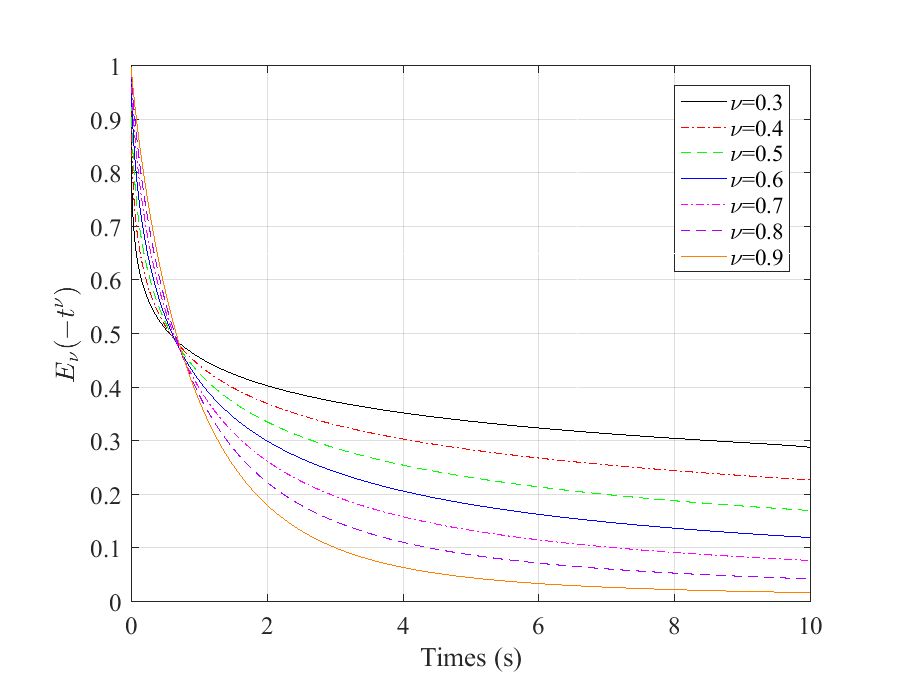
\includegraphics[scale=0.5]{p9_Ev.eps}               
\end{minipage}
}
\subfigure[Trajectories of of $t^{\nu-1}E_{\nu,\nu}\left(-t^\nu\right)$]
{                    
  \begin{minipage}{7cm}
    \centering                                                          
  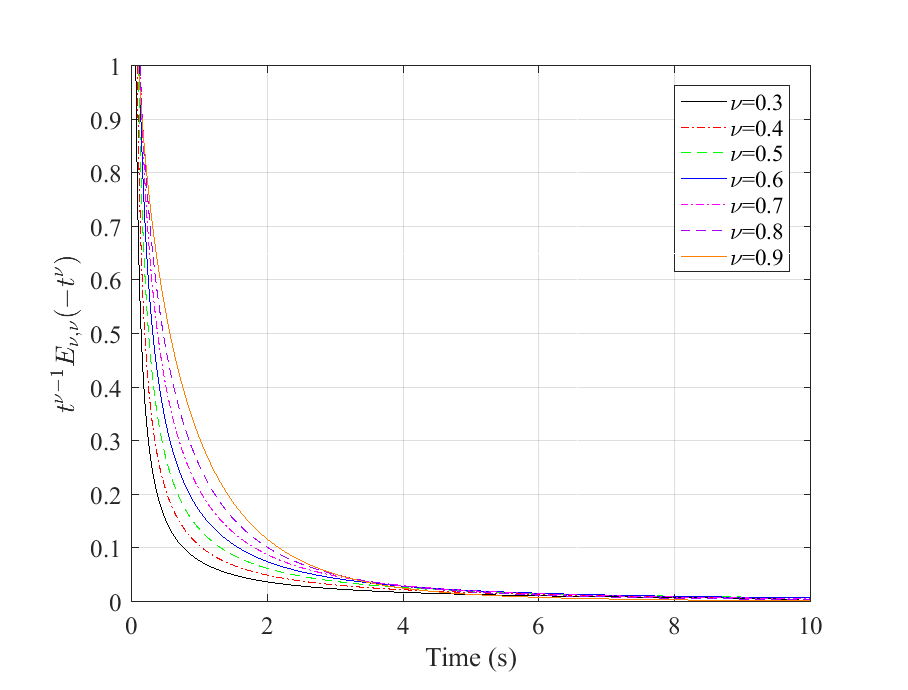
\includegraphics[scale=0.5]{p9_Evv.eps}                
\end{minipage}
}\caption{Mittag--Leffler function} 
\label{fig:Ev}                                                        
\end{figure}

Moreover, the monotonicity of exponent-like Mittag--Leffler function results in the boundedness of Eq.(\ref{eq:solution fo UUB}), and trajectories of functions $E_{\nu,\nu}\left(-t^\nu\right)$ and $t^{\nu-1}E_{\nu,\nu}\left(-t^\nu\right)$ are illustrated in Fig~\ref{fig:Ev}. It indicates that the second term on the right side $\vert g(t)\vert\left[t^{\nu-1}E_{\nu,\nu}\left(-\frac{\alpha_3}{\alpha_2}t^\nu\right)\right]$ will converge to a small vicinity of origin with $t\to\infty$. Due to bounded $g(t)$ and Mittag--Leffler function, it is easy to find $T_g<\infty$ satisfying $V(t)<\xi$ when $t>T_g$, where $\xi>\vert g(t)\vert$.

Based on Eq.(\ref{eq:ML UUB}) and $V(t)<\xi,t>T_g$, it follows
\begin{align*}
  &\alpha_1\Vert\bm x\Vert^a< \xi,\ t>T_g\\
  \Rightarrow&\Vert\bm x\Vert<\left(\frac{\xi}{\alpha_1}\right)^\frac{1}{a},\ t>T_g
\end{align*}
for $t>T_g$, one has $\Vert\bm x\Vert<\left(\frac{\xi}{\alpha_1}\right)^\frac{1}{a}$, implying $\bm x$ is uniformly ultimately bounded. 

It completes the proof.
\end{proof}


\begin{myrem}
  It is noted that, Theorem~\ref{theorem:fo UUB} utilizes Caputo fractional order calculus to indicate the uniform ultimate boundedness of fractional order systems, and Riemann--Liouville fractional order calculus can be synthesized with Theorem~\ref{theorem:fo UUB} by the following lemma.
\end{myrem}

\begin{mylem}\label{lemma:C RL ineq}\cite{Li2009}
  Considering $\nu\in(0,1)$ and $M(t)$ with $M(0)\ge 0$, one has the relation between Caputo and Riemann--Liouville fractional order calculus ${}^C_{t_0}D^\nu_t M(t)\le {}^{RL}_{\ t_0}D^\nu_t M(t)$.
\end{mylem}
\begin{mythm}\label{theorem:foD UUB}
  If a nonlinear system meets the condition in Theorem~\ref{theorem:fo UUB}, it is capable of replacing Caputo fractional order operator $^C D$ with Riemann--Liouville fractional order operator $D$ to obtain the same result.
\end{mythm}
\begin{proof}
  Considering $\bm x$ and Lyapunov function candidate $V(t,\bm x)$, 
  \begin{align}
      \begin{split}\label{eq:ML UUB RL}
      &\alpha_1\Vert\bm x\Vert^a\le V(t,\bm x(t))\le\alpha_2\Vert\bm x\Vert^{ab}\\
       &D^\nu V(t,\bm x(t))\le-\alpha_3\Vert\bm x\Vert^{ab}+g(t)
    \end{split}
    \end{align}
  if the following inequality exists
  \begin{align*}
      D^\nu V(t,\bm x(t))\le -\frac{\alpha_3}{\alpha_2}V(t,\bm x(t))+g(t),
  \end{align*}
  due to $V(0)\ge 0$ and Lemma \ref{lemma:C RL ineq}, one has
  \begin{align*}
      ^C_{t_0} D^\nu_t V(t,\bm x(t))\le D^\nu V(t,\bm x(t))\le-\frac{\alpha_3}{\alpha_2}V(t,\bm x(t))+g(t).
  \end{align*}
  Referred to the analyses in Theorem \ref{theorem:fo UUB}, $V(t,\bm x)$ and $\bm x$ are uniformly ultimately bounded. 
  
  This completes the proof.
\end{proof}

The fractional order sliding surface contains fractional derivate and integral of integer-order sliding surface as follows:
\begin{align}
  s_{fo}&=D^{1-\nu}s+D^{-\nu}s,\label{eq:sfo}
\end{align}
and fractional order disturbance observers can be described by
\begin{align}\begin{split}
  \hat d_3 &= D^{1-\nu}q_3+k_6D^{1-\nu}e_2\\
  \dot q_3 &= -k_6D^{1-\nu}q_3-k_6(f_1+k_6D^{1-\nu}e_2)\label{eq:fodo1}
\end{split}\\\begin{split}
  \hat d_4 &= D^{1-\nu}q_2+k_7D^{1-\nu}e_4\\
  \dot q_4 &= -k_7D^{1-\nu}q_2-k_7(f_2+u+k_7D^{1-\nu}e_4).\label{eq:fodo2}
\end{split}\end{align}

To deal with the input limitation in Eq.(\ref{eq:nominal model}), a novel fractional order auxiliary variable is presented as follows:
\begin{align}
\eta_{fo}=\left\{
\begin{aligned}
&-D^{-\nu}\left(k_9\eta_{fo}+\frac{(\partial f_1/\partial e_4)s_{fo}\Delta u+\frac{1}{2}\Delta u^2}{\eta_{fo}^2}\eta_{fo}-\Delta u\right),\quad&\vert\eta_{fo}\vert\ge\sigma \\
&0,\quad&\vert\eta_{fo}\vert<\sigma \end{aligned}
\right.\label{eq:adaptionfo}
\end{align}
\begin{myrem}
  Lemma~\ref{lem: adaptive input} presents an integer-order adaptive law which is modified to a fractional order version. The fractional order adaptive law is a part of the control command to deal with input limitation in tension control for the deployment of TSS.  
\end{myrem}
Hence the fractional order sliding mode controller can be designed according to the following theorem.

\begin{mythm}
  Considering system (\ref{eq:nominal model}) representing the deployment dynamics of TSS with input constraint and external disturbance, in the light of $\eta_{fo}=D^{1-\nu}\eta$, Eq.(\ref{eq:fodo1}) and Eq.(\ref{eq:fodo2}), a fractional order sliding mode control law can be constructed as
  \begin{align}\begin{split}
    u_c =& -\left(\frac{\partial f_1}{\partial e_4}\right)^{-1}\left(s+c_1e_2+c_2f_1+\frac{\partial f_1}{\partial e_1}e_2+\frac{\partial f_1}{\partial e_2}f_1+\frac{\partial f_1}{\partial e_3}e_4+\frac{\partial f_1}{\partial e_4}f_2\right)\\
    &-\left(\frac{\partial f_1}{\partial e_4}\right)^{-1}k_8s_{fo}-\hat d_4-\left(\frac{\partial f_1}{\partial e_4}\right)^{-1}\left(c_2+\frac{\partial f_1}{\partial e_2}\right)\hat d_3-k_{10}\left(\frac{\partial f_1}{\partial e_4}\right)^{-1}\eta_{fo}\label{eq:fouc}
  \end{split}\end{align}
  to ensure all the system state errors are uniformly ultimately bounded.
\end{mythm}
\begin{proof}
  Select the Lyapunov function candidate
  \begin{align}
    V_{fo}=s_{fo}^2+\tilde d_3^2+\tilde d_4^2+\eta_{fo}^2.\label{eq:vfo}
  \end{align}

  Using Lemma \ref{lem:v}, the $\nu$-th derivative of $V_{fo}$ results in
  \begin{align}\begin{split}
    D^\nu V_{fo}\le& s_{fo}D^\nu s_{fo}+\tilde d_3D^\nu \tilde d_3+\tilde d_4D^\nu \tilde d_4+\eta_{fo}D^\nu \eta_{fo}
    \\&+\vartheta_1\vert s_{fo}\vert+\vartheta_2\vert \tilde d_3\vert+\vartheta_3\vert \tilde d_4\vert+\vartheta_4\vert \eta_{fo}\vert.\label{eq:Dv}
  \end{split}\end{align}
  In the view of Eqs.(\ref{eq:sfo}-\ref{eq:fouc}), one has
  \begin{align}\begin{split}
    s_{fo}D^\nu s_{fo}&=s_{fo}(\dot s+s)\\
    &=s_{fo}\left[-k_8s_{fo}-\left(\frac{\partial f_1}{\partial e_4}\right)\hat d_4+\left(\frac{\partial f_1}{\partial e_4}\right)d_2-\left(c_2+\frac{\partial f_1}{\partial e_2}\right)\hat d_3+\left(c_2+\frac{\partial f_1}{\partial e_2}\right)d_1+\frac{\partial f_1}{\partial e_4}\Delta u-k_{10}\eta_{fo}\right]\\
    &=-k_8s_{fo}^2+\left(\frac{\partial f_1}{\partial e_4}\right)s_{fo}\tilde d_4 +\left(c_2+\frac{\partial f_1}{\partial e_2}\right)s_{fo}\tilde d_3+\frac{\partial f_1}{\partial e_4}s_{fo}\Delta u-k_{10}\eta_{fo} s_{fo}\\
    &\le -k_8s_{fo}^2+\frac{1}{2}\left(\frac{\partial f_1}{\partial e_4}\right)^2s_{fo}^2+\frac{1}{2}\tilde d_4^2+\frac{1}{2}\left(c_2+\frac{\partial f_1}{\partial e_2}\right)^2s_{fo}^2+\frac{1}{2}\tilde d_3^2+\frac{1}{2}s_{fo}^2+\frac{1}{2}k_{10}^2\eta_{fo}^2+\frac{\partial f_1}{\partial e_4}s_{fo}\Delta u\\
    &\le -\left[k_8-\frac{1}{2}-\frac{1}{2}\left(c_2+\frac{\partial f_1}{\partial e_2}\right)^2-\frac{1}{2}\left(\frac{\partial f_1}{\partial e_4}\right)^2\right]s_{fo}^2+\frac{1}{2}\tilde d_4^2+\frac{1}{2}\tilde d_3^2+\frac{1}{2}k_{10}^2\eta_{fo}^2+\frac{\partial f_1}{\partial e_4}s_{fo}\Delta u.\label{eq:sDs}
  \end{split}\end{align}
  According to $\tilde d_3 = \hat d_3 - d_1$, Eq.(\ref{eq:fodo1}), Assumption \ref{as:2} and Young's inequality, one has
  \begin{align}\begin{split}
    \tilde d_3D^\nu \tilde d_3&=\tilde d_3\left(D^\nu\hat d_3-D^\nu d_1\right)\\
    &=\tilde d_3\left(\dot q_3+k_6\dot e_2-D^\nu d_1\right)\\
    &=\tilde d_3\left[-k_6D^{1-\nu}q_3-k_6(f_1+k_6D^{1-\nu}e_2)+k_6(f_1+d_1)-D^\nu d_1\right]\\
    &=\tilde d_3\left[-k_6(D^{1-\nu}q_3+k_6D^{1-\nu}e_2-d_1)-D^\nu d_1\right]\\
    &=-k_6\tilde d_3^2-\tilde d_3D^\nu d_1\\
    &\le-\left(k_6-\frac{1}{2}\right)\tilde d_3^2+\frac{1}{2}\rho_5^2\label{eq:d3d3}
  \end{split}\end{align}
  and along the same line, one can also obtain
  \begin{align}
    \tilde d_4D^\nu \tilde d_4 \le-\left(k_7-\frac{1}{2}\right)\tilde d_4^2+\frac{1}{2}\rho_6^2\label{eq:d4d4}
  \end{align}
  Similar to the integral sliding mode controller, the overall stability analysis will be divided into two cases based on the region which $\eta_{fo}$ locates in.
  \begin{mycase1}
    When $\vert\eta_{fo}\vert\ge\sigma$, introducing Eq.(\ref{eq:adaptionfo}), Eq.(\ref{eq:sDs}), Eq.(\ref{eq:d3d3}) and Eq.(\ref{eq:d4d4}) into Eq.(\ref{eq:Dv}) obtains
    \begin{align}\begin{split}
      D^\nu V_{fo} \le &-\left[k_8-\frac{1}{2}-\frac{1}{2}\left(c_2+\frac{\partial f_1}{\partial e_2}\right)^2-\frac{1}{2}\left(\frac{\partial f_1}{\partial e_4}\right)^2\right]s_{fo}^2-\left(k_6-1\right)\tilde{d}_3^2-\left(k_7-1\right)\tilde{d}_4^2\\
      &-\left(k_9-\frac{1}{2}k_{10}^2-\frac{1}{2}\right)\eta_{fo}^2+\frac{1}{2}\rho_5^2 +\frac{1}{2}\rho_6^2+\vartheta_1\vert s_{fo}\vert+\vartheta_2\vert \tilde d_3\vert+\vartheta_3\vert \tilde d_4\vert+\vartheta_4\vert \eta_{fo}\vert\\
      \le &-\left[k_8-1-\frac{1}{2}\left(c_2+\frac{\partial f_1}{\partial e_2}\right)^2-\frac{1}{2}\left(\frac{\partial f_1}{\partial e_4}\right)^2\right]s_{fo}^2-\left(k_6-\frac{3}{2}\right)\tilde{d}_3^2-\left(k_7-\frac{3}{2}\right)\tilde{d}_4^2\\
      &-\left(k_9-\frac{1}{2}k_{10}^2-1\right)\eta_{fo}^2+\frac{1}{2}\rho_5^2 +\frac{1}{2}\rho_6^2+\frac{1}{2}\vartheta_1^2+\frac{1}{2}\vartheta_2^2+\frac{1}{2}\vartheta_3^2+\frac{1}{2}\vartheta_4^2\\
      \le& -\xi_1V+\Psi_1.
    \end{split}\end{align}
    where
    \begin{align}\begin{split}
      \xi_1 &= \min\left\{k_8-1-\frac{1}{2}\left(c_2+\frac{\partial f_1}{\partial e_2}\right)^2-\frac{1}{2}\left(\frac{\partial f_1}{\partial e_4}\right)^2,k_6-\frac{3}{2},k_7-\frac{3}{2},k_9-\frac{1}{2}k_{10}^2-1\right\}>0\\
      \Psi_1&=\frac{1}{2}\rho_5^2 +\frac{1}{2}\rho_6^2+\frac{1}{2}\vartheta_1^2+\frac{1}{2}\vartheta_2^2+\frac{1}{2}\vartheta_3^2+\frac{1}{2}\vartheta_4^2.
    \end{split}\end{align}
  \end{mycase1}
  \begin{mycase1}
    When $\vert\eta_{fo}\vert<\sigma$, introducing Eq.(\ref{eq:adaptionfo}), Eq.(\ref{eq:sDs}), Eq.(\ref{eq:d4d4}) and Eq.(\ref{eq:d3d3}) into Eq.(\ref{eq:Dv}) obtains
    \begin{align}\begin{split}
      D^\nu V_{fo} \le&-\left[k_8-\frac{1}{2}-\frac{1}{2}\left(c_2+\frac{\partial f_1}{\partial e_2}\right)^2-\left(\frac{\partial f_1}{\partial e_4}\right)^2\right]s_{fo}^2-\left(k_6-1\right)\tilde{d}_3^2-\left(k_7-1\right)\tilde{d}_4^2\\
      &-\frac{1}{2}k_{10}^2\eta_{fo}^2+\frac{1}{2}\Delta u^2+\frac{1}{2}\rho_5^2+\frac{1}{2}\rho_6^2+\vartheta_1\vert s_{fo}\vert+\vartheta_2\vert \tilde d_3\vert+\vartheta_3\vert \tilde d_4\vert+\vartheta_4\vert \eta_{fo}\vert\\
      \le&-\left[k_8-1-\frac{1}{2}\left(c_2+\frac{\partial f_1}{\partial e_2}\right)^2-\left(\frac{\partial f_1}{\partial e_4}\right)^2\right]s_{fo}^2-\left(k_6-\frac{3}{2}\right)\tilde{d}_3^2-\left(k_7-\frac{3}{2}\right)\tilde{d}_4^2\\
      &-(\frac{1}{2}k_{10}^2-\frac{1}{2})\eta_{fo}^2+\frac{1}{2}\sigma^2+\frac{1}{2}\rho_5^2+\frac{1}{2}\rho_6^2+\frac{1}{2}\vartheta_1^2+\frac{1}{2}\vartheta_2^2+\frac{1}{2}\vartheta_3^2+\frac{1}{2}\vartheta_4^2\\
      \le& -\xi_2V+\Psi_2
    \end{split}\end{align}
    where
    \begin{align}\begin{split}
      \xi_2&=\min\left\{k_8-1-\frac{1}{2}\left(c_2+\frac{\partial f_1}{\partial e_2}\right)^2-\left(\frac{\partial f_1}{\partial e_4}\right)^2,k_6-\frac{3}{2},k_7-\frac{3}{2},\frac{1}{2}k_{10}^2-\frac{1}{2}\right\}>0\\
      \Psi_2&=\frac{1}{2}\sigma^2+\frac{1}{2}\rho_5^2+\frac{1}{2}\rho_6^2+\frac{1}{2}\vartheta_1^2+\frac{1}{2}\vartheta_2^2+\frac{1}{2}\vartheta_3^2+\frac{1}{2}\vartheta_4^2.
    \end{split}\end{align}
  \end{mycase1}
  Therefore, one has
  \begin{align}\begin{split}
    D^\nu V_{fo}&\le-\xi V_{fo}+\Psi.
  \end{split}\end{align}
  According to Theorem~\ref{theorem:foD UUB}, $V_{fo}$ and $s_{fo}$ are uniformly ultimately bounded. Therefore, one can proceed to prove that all the system state errors are uniformly ultimately bounded by referring to the deduction from Eq.(\ref{eq:abs s}) to Eq.(\ref{eq:sigma2}), which is omitted here. 
  
  This completes the proof.
\end{proof}

\section{Numerical simulations}\label{sec:numerical simulation}
To verify the effectiveness of the proposed nonlinear fractional order sliding mode controller for deployment dynamics of TSS, numerical simulations are carried out in this section.

Firstly, The simulation parameters including the orbital parameters and physical properties of the space tether are presented, and we select the conditions of YES2 phase 1 deployment task as the reference, where mother spacecraft mass is 6530 {kg} and Subspacecraft mass is 12 {kg}. Accordingly, this work will deploy 3.5 {km} of space tether, and the space tether should maintain as close to the local vertical as possible during the task. The orbital altitude of the TSS running is approximate to 260 {km}, and it is reasonable to assume that the true anomaly is 0 {rad} when ejecting the space tether and subspacecraft from mother spacecraft. Therefore the initial length of the space tether between the subspacecraft and the mother spacecraft is set as 3 {m}. The ejection speed of the subspacecraft is 1.25 {m/s}, and the initial inplane angle is described by the following conditions: $\theta_0=0.01$ {rad} and $\dot\theta_0 = 0$ {rad/s}. Without loss of generality external disturbance can be expressed by a periodical function $d_2=1\times 10^{-2}\sin(\nu)$ N. Based on theses conditions, the initial state of the entire dimensionless system can be expressed approximatively: $\lambda_0 =9\times 10^{-4},\dot\lambda_0=0.3,\theta_0 = 0.01,\dot\theta_0=0$, and the desired state follows: $\lambda_d =1,\dot\lambda_d=0,\theta_d = 0,\dot\theta_d=0$, indicating the deployment  has been finished. 

It is well known that the space tether can not be compressed like a stick while the tension beyond the maximum tolerance will lead to the fragmentation,
Physically, the tension along the space tether should be positive to ensure the space tether tightened, the constrained input of the system can be calculated with Eq.(\ref{eq:varcon}). selecting a very small $\tau_{min} = 10^{-6}$ \textit{N} to guarantee the space tether taut and straight during the task, and the assumed dimensionless tension: $10^{-3}\le\hat{\tau}\le 10$. The linearization result exhibits a relevant explicit form of the system input: $u = - \hat{\tau}$, thus one can obtain input limitation: $-10\le u\le-10^{-3}$, making the system meet the realistic situation. 

According to the proposed integer-order controller design, to ensure the existence of sliding surface, time-varying parameters of controller and observer can be designed as follows:
\begin{align*}
    k_1=&{\max}\left\{\frac{1}{2}+\frac{1}{2}\left\vert c_2+\frac{\partial f_1}{\partial {\dot e_1}}\right\vert+\varrho/100,\varrho\right\}\\
    k_2=&{\max}\left\{\frac{1}{2}+\frac{1}{2}\left\vert\frac{\partial f_1}{\partial {\dot e_2}}\right\vert+\varrho/100,\varrho\right\},\\
    k_3=&{\max}\left\{\frac{1}{2}+\frac{1}{2}k_5^2+\varrho/100,\varrho\right\},\ k_5=10,\\
    k_4=&{\max}\left\{\frac{1}{2}\left\vert c_2+\frac{\partial f_1}{\partial {\dot e_1}}\right\vert+\frac{1}{2}\left\vert\frac{\partial f_1}{\partial {\dot e_2}}\right\vert+\frac{1}{2}\left(\frac{\partial f_1}{\partial {\dot e_2}}\right)^2+\frac{1}{2}+\varrho/100,\right.\\
    &\left.\frac{1}{2}\left\vert c_2+\frac{\partial f_1}{\partial {\dot e_1}}\right\vert+\frac{1}{2}\left\vert\frac{\partial f_1}{\partial {\dot e_2}}\right\vert+\frac{1}{2}+\varrho/100,\varrho\right\}
\end{align*}
where $\varrho$ is a constant, without loss of generality, one can select $\varrho=100$, $\eta(0)=100$ and $\sigma=0.01$ to obtain a satisfactory performance. Similarly, the parameters of the fractional order controller can be selected as $k_6=10$, $k_7=10$, $k_9=5$, $k_{10}=2$ and
\begin{align*}
    k_8=&{\max}\left\{1+\frac{1}{2}\left(c_2+\frac{\partial f_1}{\partial {\dot e_1}}\right)^2+\frac{1}{2}\left(\frac{\partial f_1}{\partial \dot e_2}\right)^2+\varrho/100,\right.\\
    &\left.1+\frac{1}{2}\left(c_2+\frac{\partial f_1}{\partial {\dot e_1}}\right)^2+\left(\frac{\partial f_1}{\partial \dot e_2}\right)^2+\varrho/100,\varrho\right\}.
\end{align*}

Parameters of sliding surface can be chosen as $c_1=75$, $c_2=3$ and $\varepsilon=35$ to guarantee that the reduced order system is uniformly ultimately bounded.
 
Figures~\ref{fig:compare_length} and~\ref{fig:compare_theta} illustrate the comparison between nonlinear sliding mode control for deployment of TSS in Ref.~\cite{Ma2017Pure} and integral sliding mode control which is proposed in this paper. In the dynamic phase, the space tether length trajectory of integral method rise more smoothly than the nonlinear method, and reaches the desired value earlier without any overshoot. In the steady phase, the integral method has smaller steady errors, and contrarily, the trajectory of nonlinear method fluctuates around the desired value. Figure~\ref{fig:compare_theta} shows that the integral method performs a greater swing of the space tether and completes a faster deployment with smaller steady errors than the nonlinear method. 

\begin{figure}[hbtp]
  \centering
  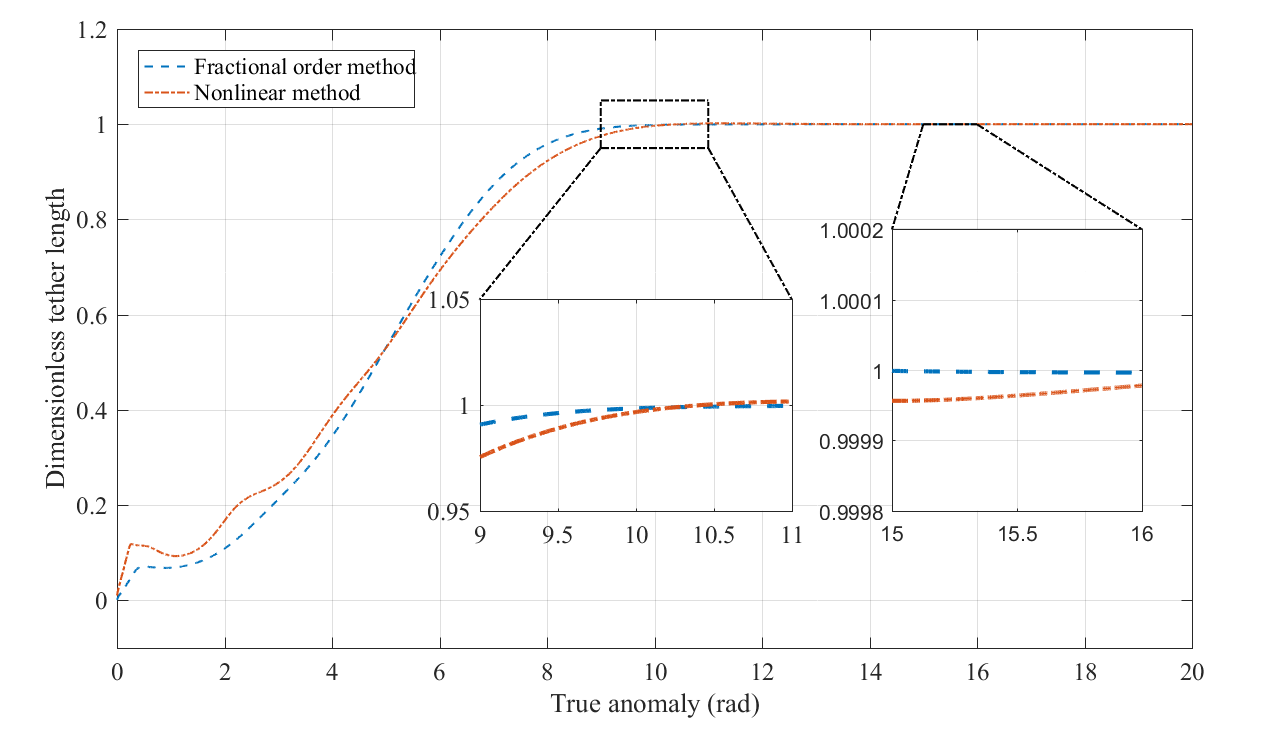
\includegraphics[width=0.8\textwidth]{p9_compare_length.eps}
  \caption{Trajectories of dimensionless tether length compared with nonlinear sliding mode control}
  \label{fig:compare_length}
  \end{figure}
  \begin{figure}[hbtp]
    \centering
    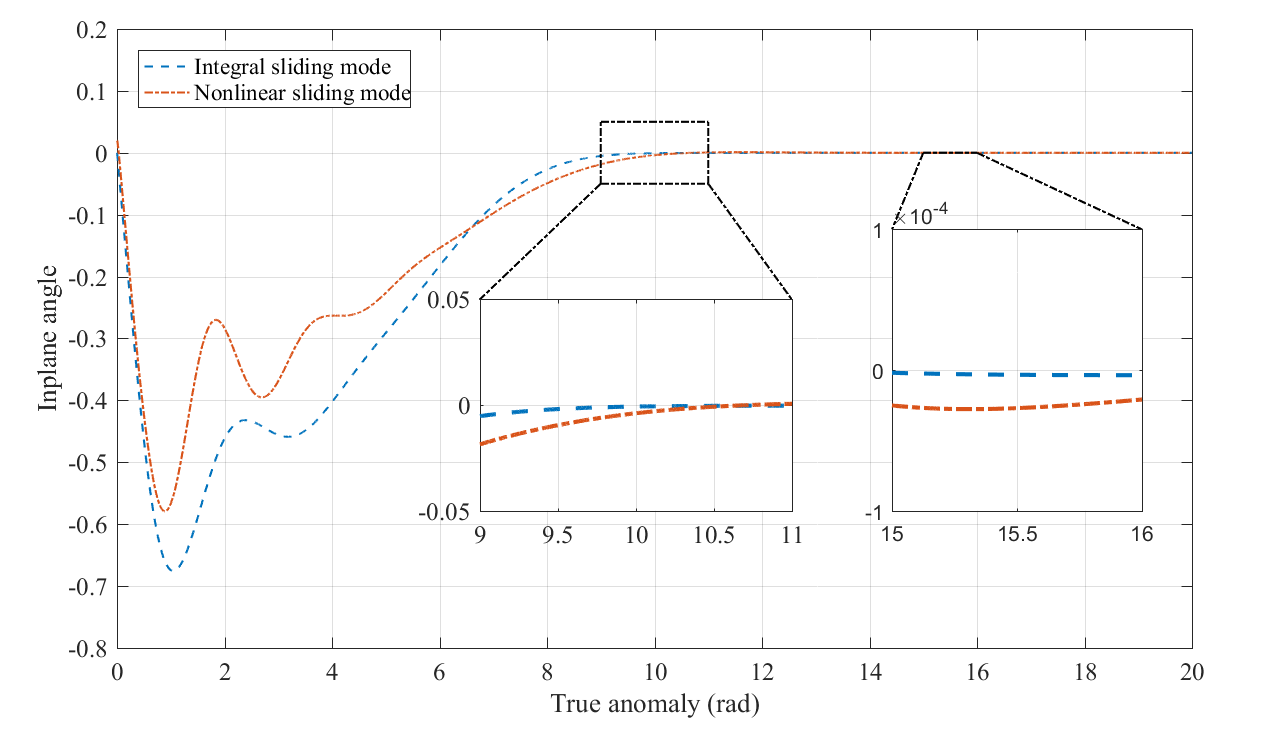
\includegraphics[width=0.8\textwidth]{p9_compare_theta.eps}
    \caption{Trajectories of inplane angle compared with nonlinear sliding mode control}
    \label{fig:compare_theta}
    \end{figure}

    
The integral sliding mode control can be viewed as a special fractional order sliding mode control with order $\nu=1$. Its length and inplane angle trajectories are also drawn in Figures~\ref{fig:length} and~\ref{fig:angle}, and simulation results indicate that the controllers with fractional order $0<\nu<1$ perform better. Furthermore, it concludes that the proposed methods in this paper work more effective than the method in Ref.~\cite{Ma2017Pure}.

\begin{figure}[hbtp]
  \centering
  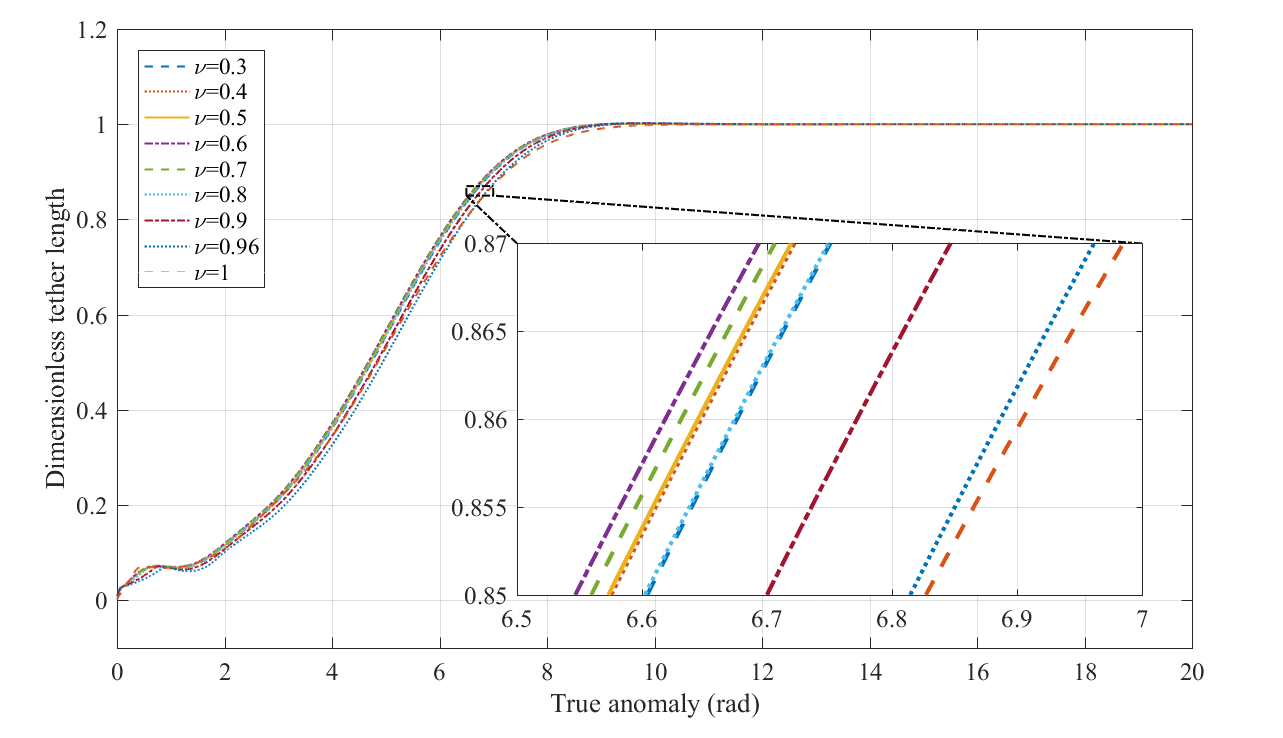
\includegraphics[width=0.8\textwidth]{p9_length.eps}
  \caption{Trajectories of dimensionless tether length}
  \label{fig:length}
  \end{figure}

  Figure~\ref{fig:length} shows the dynamics of the length during the deployment, and it is obvious from the simulation results that there exist a cluster of trajectories expressing the deployment dynamics with different fractional order parameters. It is hard to find the overshoot from this cluster of trajectories while the proposed fractional order sliding mode controllers can guarantee a smooth and fast deployment subjected to pure tension. 
  
  The difference fractional order parameter will result in gradual varying performance that can be seen in the enlarged figures. Because the fractional order sliding mode controller is consisting of fractional derivate and integral operators, the interaction is reflected in the simulation results, and one can find $\nu =0.5$, $\nu=0.6$ and $\nu=0.7$ produce the better performance than other order parameters, and the performance improves as the parameter increases when $\nu\le 0.5$ while the performance degenerates as the parameter decreases when $\nu> 0.5$. 

  It is noted that we specify the order parameter as $\nu=0.96$ approximating to an integer-order sliding mode controller, and from the simulation results, one can find that they have the similar performance but the fractional order one is better.
  \begin{figure}[hbtp]
    \centering
    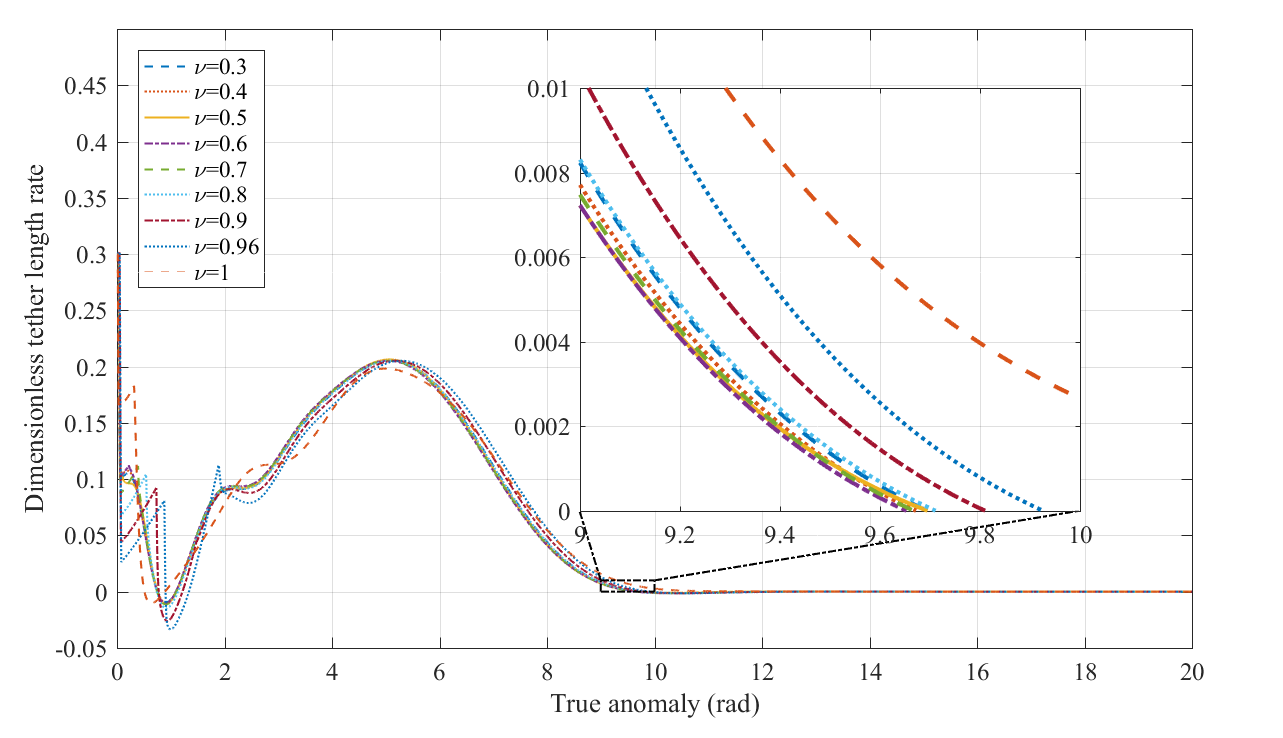
\includegraphics[width=0.8\textwidth]{p9_length_rate.eps}
    \caption{Trajectories of dimensionless tether length rate}
    \label{fig:length rate}
    \end{figure} 

One can see the simulation results of the dynamics of space tether length rate from Figure~\ref{fig:length rate}, and some negative length rates can be found during the deployment which are not desired, because this phenomena means that the reel of space tether is working instead of the brake device. From the enlarged figure, the results are similar to Figure~\ref{fig:length}, the performance with the order parameters around $\nu =0.5$ are much better. 
%width=10cm,height=7cm
\begin{figure}[hbtp]
  \centering
  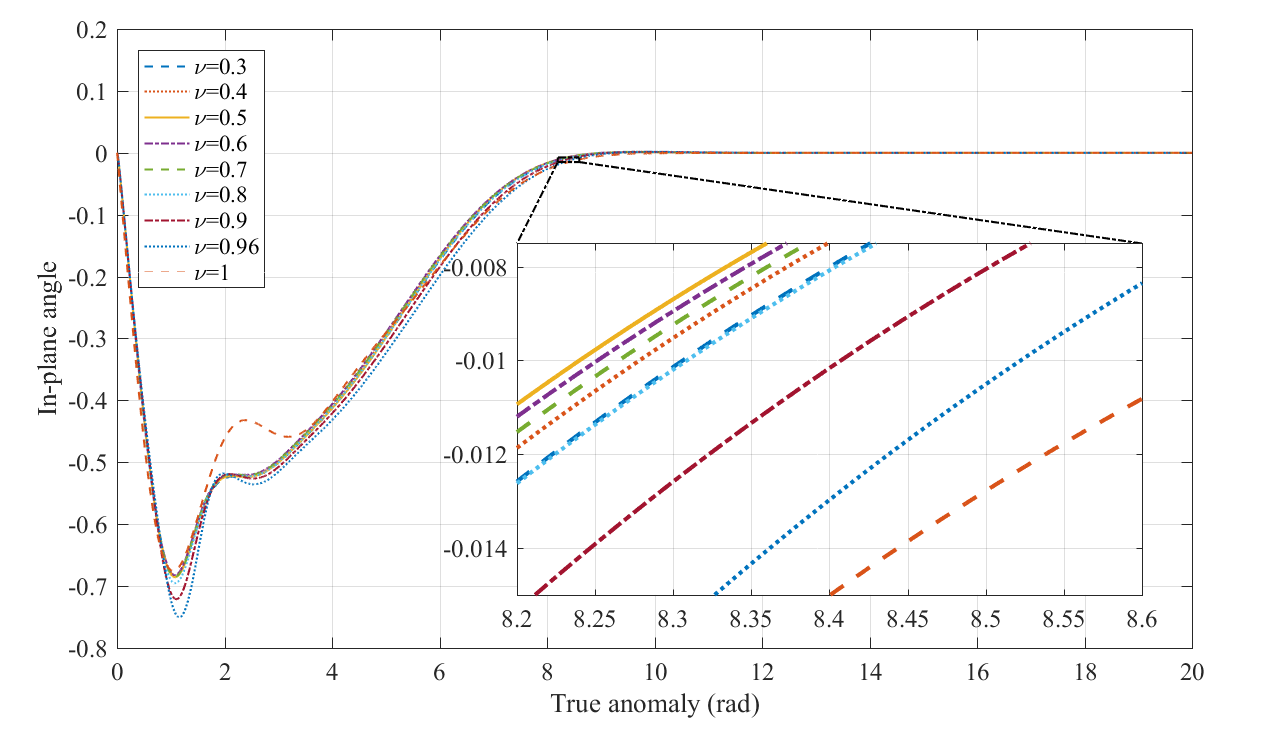
\includegraphics[width=0.8\textwidth]{p9_angle.eps}
  \caption{Trajectories of inplane angle}
  \label{fig:angle}
  \end{figure}

  Figure~\ref{fig:angle} shows the dynamics of the inplane angle, and it is reasonable to say the deployment will be completed at 10 {\it rad} with the results shown in Figure~\ref{fig:length}. The varying regions of the inplane angles are feasible which will not lead to a great swing of the space tether. The results also indicate the derivation caused by the gradual order parameters. The best performances appear when the order parameters are selected around $\nu =0.5$, and moreover all the results with fractional order are better than the integer-order one. 
\begin{figure}[hbtp]
  \centering
  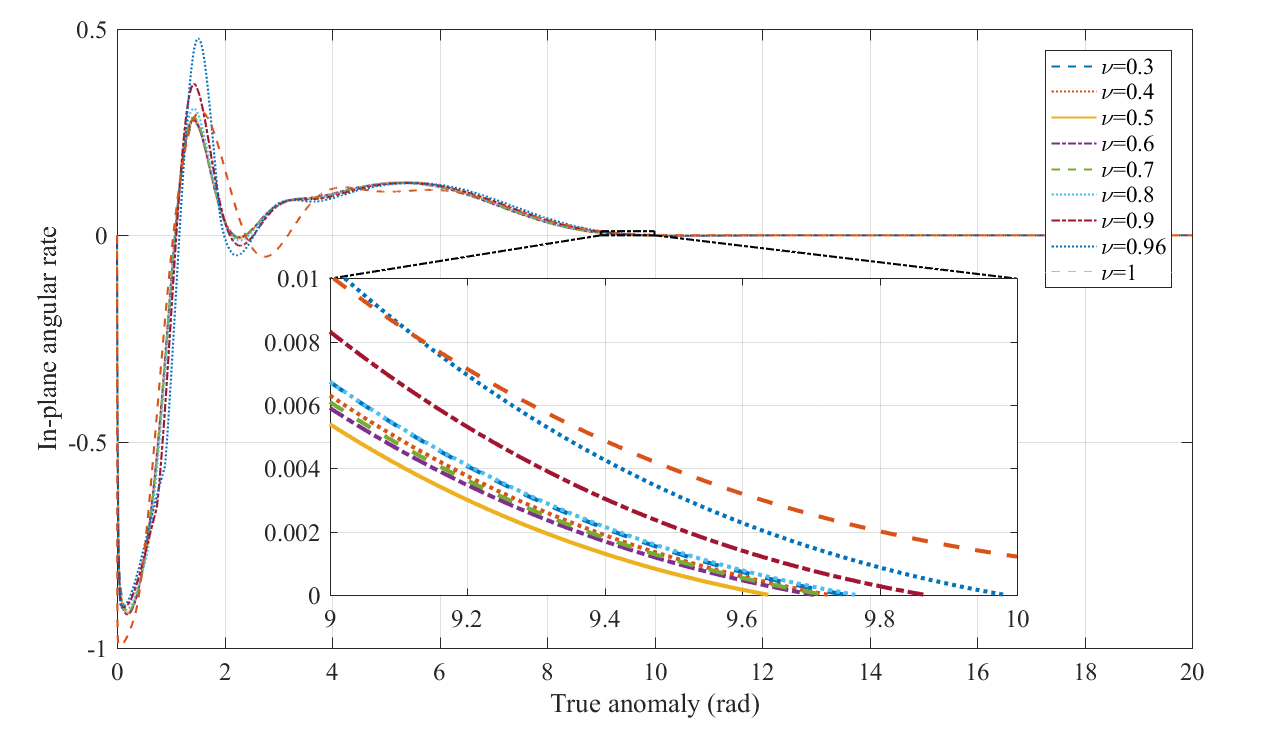
\includegraphics[width=0.8\textwidth]{p9_angular_rate.eps}
  \caption{Trajectories of inplane angular rate} 
  \label{fig:angular rate}
  \end{figure}

  Figure~\ref{fig:angular rate} shows the dynamics of the inplane angle rate, and it is worth mentioning that all the values satisfy the assumption about the controller design, which will not cause any singularity in the control laws based on the nonlinear fractional order sliding surface. One can see a fine tuning after 10 {\it rad} at the level of $10^{-3}$ when the deployment is finishing. 
  \begin{figure}[hbtp]
    \centering
    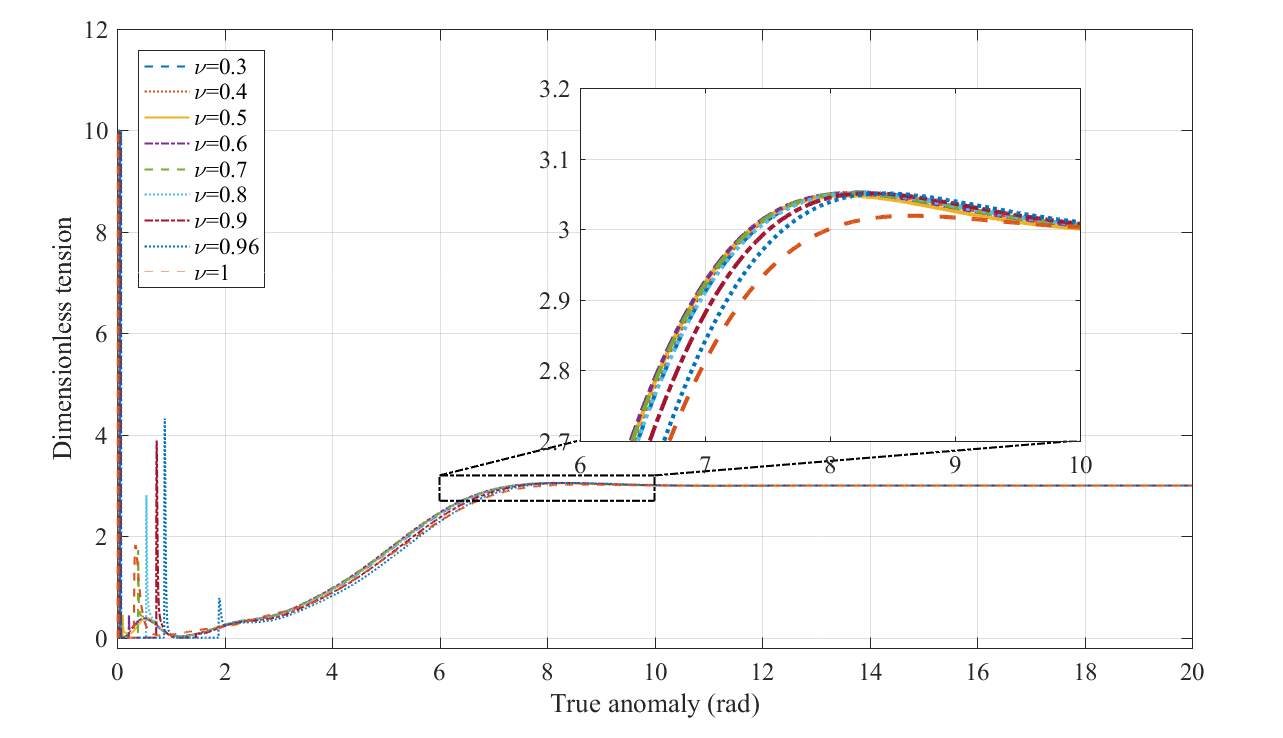
\includegraphics[width=0.8\textwidth]{p9_input.eps} 
    \caption{Trajectories of dimensionless tension}
    \label{fig:input}
    \end{figure}

   The trajectories of tension are illustrated in Figure~\ref{fig:input}, from which it is obvious that there is not any negative value occurring during the deployment, indicating that all the inputs during the deployment are feasible, and the final stable values are equivalent to 3 that is coincident with the reality.
 
   There do not exist obvious fluctuations in the stable states of all these trajectories because of the disturbance eliminating external disturbances. 
\section{Conclusion}\label{sec:Conclusion} 
This paper has proposed a nonlinear fractional order sliding mode control scheme for the deployment of TSS with pure tension. A fractional order adaptive law has been developed to remove the adverse effect in the stability analysis. Fractional order uniform ultimate boundedness has been proved based on Mittag-Leffler stability theory. A fractional order sliding surface is designed to integrate the integer-order and fractional order sliding surfaces into a united frame, and the controller parameter guidance aids control precision enhancement. Compared with existing integer-order sliding mode control methods, the proposed fractional order method has better performance in both dynamic and steady phases. The simulation results show the performance of the fractional order sliding mode control is dependent on the selection of order parameter. This fractional order method has the potential to be utilized in regulating three-dimensional motions of TSS, which will be reported in our future paper. 
\section{Acknowledgment}
This work is partially supported by the National Natural Science Foundation of China (No. 61104112, 61503097).
%\section{References}
%\bibliographystyle{vancouver}
%\bibliography{paper1}
\begin{thebibliography}{10}

  \bibitem{huang_wang_meng_liu_2015}
  Huang P, Wang D, Meng Z, Liu Z.
  \newblock Post-capture attitude control for a tethered space robot-target
    combination system.
  \newblock Robotica. 2015;33(4):898--919.
  
  \bibitem{Williams2009745}
  Williams P, Hyslop A, Stelzer M, Kruijff M.
  \newblock YES2 optimal trajectories in presence of eccentricity and aerodynamic
    drag.
  \newblock Acta Astronautica. 2009;64(7):745--769.
  
  \bibitem{Steindl2016}
  Steindl A.
  \newblock Time optimal control for the deployment of a tethered satellite
    allowing for a massive tether.
  \newblock Meccanica. 2016 Nov;51(11):2741--2751.
   
  \bibitem{mantellato2017simulation}
  Mantellato R, Lorenzini E, Sternberg D, Roascio D, Saenz-Otero A, Zachrau H.
  \newblock Simulation of a tethered microgravity robot pair and validation on a
    planar air bearing.
  \newblock Acta Astronautica. 2017;138:579--589.
  
  \bibitem{ASLANOV2017180}
  Aslanov VS, Ledkov AS.
  \newblock Tether-assisted re-entry capsule deorbiting from an elliptical orbit.
  \newblock Acta Astronautica. 2017;130:180--186.
  
  \bibitem{wen2016constrained}
  Wen H, Zhu ZH, Jin D, Hu H.
  \newblock Constrained tension control of a tethered space-tug system with only
    length measurement.
  \newblock Acta Astronautica. 2016;119:110--117.
  
  \bibitem{Ma2017Pure}
  Ma Z, Sun G, Cheng Z, Li Z.
  \newblock Pure-tension non-linear sliding mode control for deployment of
    tethered satellite system.
  \newblock Proceedings of the Institution of Mechanical Engineers, Part G:
    Journal of Aerospace Engineering. 2018;232(13):2541 -- 2551.
  
  \bibitem{sun2014fractional}
  Sun G, Zhu Z.
  \newblock Fractional order tension control for stable and fast tethered
    satellite retrieval.
  \newblock Acta Astronautica. 2014;104(1):304--312.
  
  \bibitem{sun2014fractional-order}
  Sun G, Zhu Z.
  \newblock Fractional-order tension control law for deployment of space tether
    system.
  \newblock Journal of Guidance, Control, and Dynamics. 2014;37(6):2057--2062.
  
  \bibitem{yu2017analytical}
  Yu B, Jin D, Wen H.
  \newblock Analytical deployment control law for a flexible tethered satellite
    system.
  \newblock Aerospace Science and Technology. 2017;66:294--303.
  
  \bibitem{kojima2015mission}
  Kojima H, Fukatsu K, Trivailo PM.
  \newblock Mission-function control of tethered satellite/climber system.
  \newblock Acta Astronautica. 2015;106:24--32.
  
  \bibitem{wen2015space}
  Wen H, Zhu ZH, Jin D, Hu H.
  \newblock Space Tether Deployment Control with Explicit Tension Constraint and
    Saturation Function.
  \newblock Journal of Guidance, Control, and Dynamics. 2016;39(4):916--921.
  
  \bibitem{MA2017355}
  Ma Z, Sun G, Li Z.
  \newblock Dynamic adaptive saturated sliding mode control for deployment of
    tethered satellite system.
  \newblock Aerospace Science and Technology. 2017;66(Supplement C):355 -- 365.
  
  \bibitem{MA201667}
  Ma Z, Sun G.
  \newblock Adaptive sliding mode control of tethered satellite deployment with
    input limitation.
  \newblock Acta Astronautica. 2016;127(Supplement C):67 -- 75.
  
  \bibitem{zhao2018dynamic}
  Zhao Y, Huang P, Zhang F.
  \newblock Dynamic modeling and Super-Twisting Sliding Mode Control for Tethered
    Space Robot.
  \newblock Acta Astronautica. 2018;143:310--321.
  
  \bibitem{KANG2017263}
  Kang J, Zhu ZH, Wang W, Li A, Wang C.
  \newblock Fractional order sliding mode control for tethered satellite
    deployment with disturbances.
  \newblock Advances in Space Research. 2017;59(1):263 -- 273.
  
  \bibitem{Utkin1996}
  Utkin V, Shi J.
  \newblock Integral sliding mode in systems operating under uncertainty
    conditions.
  \newblock In: Proceedings of 35th IEEE Conference on Decision and Control.
    vol.~4; 1996. p. 4591--4596.

    \bibitem{sun2018practical}
    Sun G, Wu L, Kuang Z, Ma Z, Liu J.
    \newblock Practical tracking control of linear motor via fractional-order sliding mode.
    \newblock Automatica.
      2018;4: 221--235.

      \bibitem{sun2018discrete}
      Sun G, Ma Z, Yu J.
      \newblock Discrete-Time Fractional Order Terminal Sliding Mode Tracking Control for Linear Motor.
      \newblock IEEE Transactions on Industrial Electronics.
        2018;65(4): 3386--3394.

        \bibitem{sun2017practical}
        Sun G, Ma Z.
        \newblock Practical tracking control of linear motor with adaptive fractional order terminal sliding mode control.
        \newblock IEEE/ASME Transactions on Mechatronics.
          2017;22(6): 2643--2653.
  
  \bibitem{williams2008deployment}
  Williams P.
  \newblock Deployment/retrieval optimization for flexible tethered satellite
    systems.
  \newblock Nonlinear Dynamics. 2008;52(1-2):159--179.
  
  \bibitem{Do2010}
  Do KD.
  \newblock {Practical control of underactuated ships}.
  \newblock Ocean Engineering. 2010;37(13):1111--1119.
  
  \bibitem{Chen2011}
  Chen M, Ge SS, Ren B.
  \newblock {Adaptive tracking control of uncertain MIMO nonlinear systems with
    input constraints}.
  \newblock Automatica. 2011;47(3):452--465.
  
  \bibitem{Lasalle1960}
  Lasalle JP.
  \newblock {Some Extensions of Liapunov's Second Method}.
  \newblock IRE Transactions on Circuit Theory. 1960;7(4):520--527.
  
  \bibitem{Podlubny1999}
  Podlubny I, Podlubny L.
  \newblock {Fractional Differential Equations}.
  \newblock Book. 1999;p. 1--366.
  
  \bibitem{Li2009}
  Li Y, Chen Y, Podlubny I.
  \newblock Mittag–Leffler stability of fractional order nonlinear dynamic
    systems.
  \newblock Automatica. 2009;45(8):1965--1969.
  
  \bibitem{Li2010}
  Li Y, Chen Y, Podlubny I.
  \newblock {Stability of fractional-order nonlinear dynamic systems : Lyapunov
    direct method and generalized Mittag – Leffler stability}.
  \newblock Computers and Mathematics with Applications. 2010;59(5):1810--1821.
  
  \bibitem{Aghababa2014}
  Aghababa MP.
  \newblock {A Lyapunov-based control scheme for robust stabilization of
    fractional chaotic systems}.
  \newblock Nonlinear Dynamics. 2014;78(3):2129--2140.
  
  \bibitem{Miller2001Completely}
  Miller KS, Samko SG.
  \newblock Completely monotonic functions.
  \newblock Integral Transforms and Special Functions. 2001 Nov;4(12):389--402.
  
  \end{thebibliography}
  
%%%%%%%%DOCUMENT END HERE
\end{document}
